\documentclass{article}
\usepackage{amsmath}
\usepackage{mathtools}
\usepackage{gensymb}
\usepackage[a4paper,inner=1.5cm,outer=1.5cm,top=2cm,bottom=0.5cm]{geometry} 
\usepackage{xcolor}                    
\usepackage{tikz}                           
\usepackage{multicol}
\usepackage{pgfplots}
\usetikzlibrary{intersections}
\usetikzlibrary{intersections,calc,angles,quotes}
\usetikzlibrary{shapes,arrows,positioning,decorations.pathreplacing,calc}
\usetikzlibrary{calc,angles,positioning,intersections,quotes,decorations.markings}
\usepackage{tkz-euclide}
\usetikzlibrary{backgrounds}
\usetikzlibrary{calc,through}
\usetikzlibrary{angles}
\usetikzlibrary{fadings}
\usetikzlibrary{shapes.geometric}
\usetikzlibrary{shapes.symbols}
\usepackage{draftwatermark}
\usepackage{mathptmx}

\SetWatermarkText{\textcolor{black!30}{Mathema Shukur}}
\SetWatermarkFontSize{2 cm}
\usepackage[utf8]{inputenc}
\usepackage{fontspec}

\setmainfont{[Kalpurush.ttf]}
\newfontface{\en}{[Arial.ttf]} %%this is optional, if you want to use a secondary font. Any english font is supported
\newlength\Radius
\setlength\Radius{4cm}
\begin{document} 
	\Large
	\textcolor{red}{Welcome To} 
	\\
	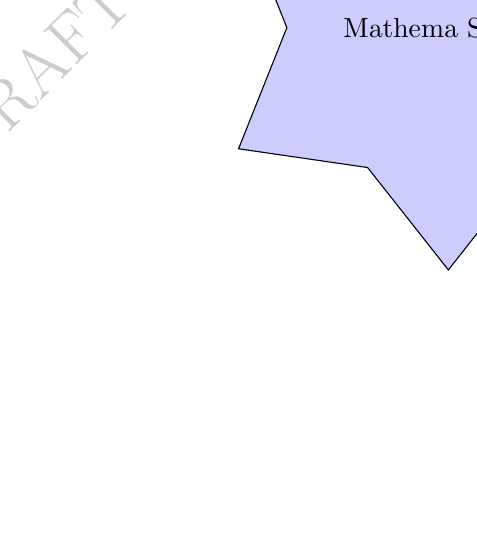
\begin{tikzpicture}
		\tikz \node [fill=blue!20,star,star points=6,draw] {Mathema Shukur };
	\end{tikzpicture}
	\\
	যাদের জন্যে প্রযোজ্যঃ  	\textcolor{magenta}{একাদশ ও দ্বাদশ শ্রেণীর শিক্ষার্থী} \\
	বিষয়ঃ \textcolor{magenta}{উচ্চতর গণিত ১ম পত্র} \\
	অধ্যায়ঃ \textcolor{magenta}{৩-সরলরেখা}\\ 
	Subtopicঃ  \textcolor{magenta}{ পোলার গ্রাফ পেপার বৃত্তাকার কেন ? }\\
	\\
	কার্তেসীয় গ্রাফ পেপার বর্গাকার\\ 
	\\ 
	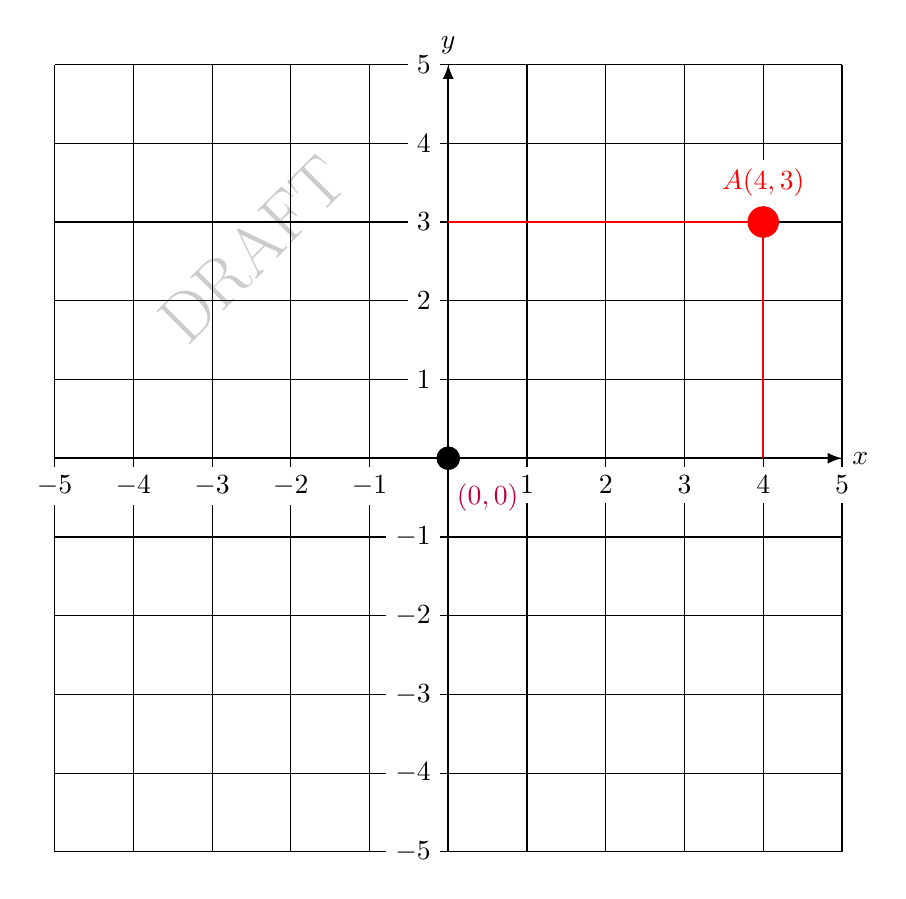
\begin{tikzpicture}[transform shape,scale=1]
		\draw (-5,-5) grid (5,5);
		\draw [-latex,thick](-5,0) -- (5,0) node[right] {$x$} coordinate(x axis);
		\foreach \x in {-5,-4,-3,-2,-1,1,2,3,4,5}
		\draw (\x,0.1) -- (\x,-0.1) node [fill=white,below] {$\x$};
		\draw [-latex,thick](0,-5) -- (0,5) node[above] {$y$} coordinate(y axis);
		\foreach \y in {-5,-4,-3,-2,-1,1,2,3,4,5}
		\draw (0.1,\y) -- (-0.1,\y) node [fill=white,left] {$\y$};
		\fill[black] (0,0) circle (1.5 mm);
		\node at (0.5,-0.5) {$\textcolor{purple}{(0,0)}$};
		\fill[red] (4,3) circle (2 mm);
	   \node[fill=white,above] at (4,3.2) {$\textcolor{red}{A(4,3)}$};
		\draw[thick,red] (4,0)--(4,3);
		\draw[thick,red] (0,3)--(4,3);
	\end{tikzpicture}
\\
$A(4,3)$ বিন্দুটিকে কার্তেসীয় গ্রাফ পেপারে প্রদর্শন করা হলো\\
\\ 
\vspace{2cm}
\\
পোলার গ্রাফ পেপার বৃত্তাকার\\ 
\\
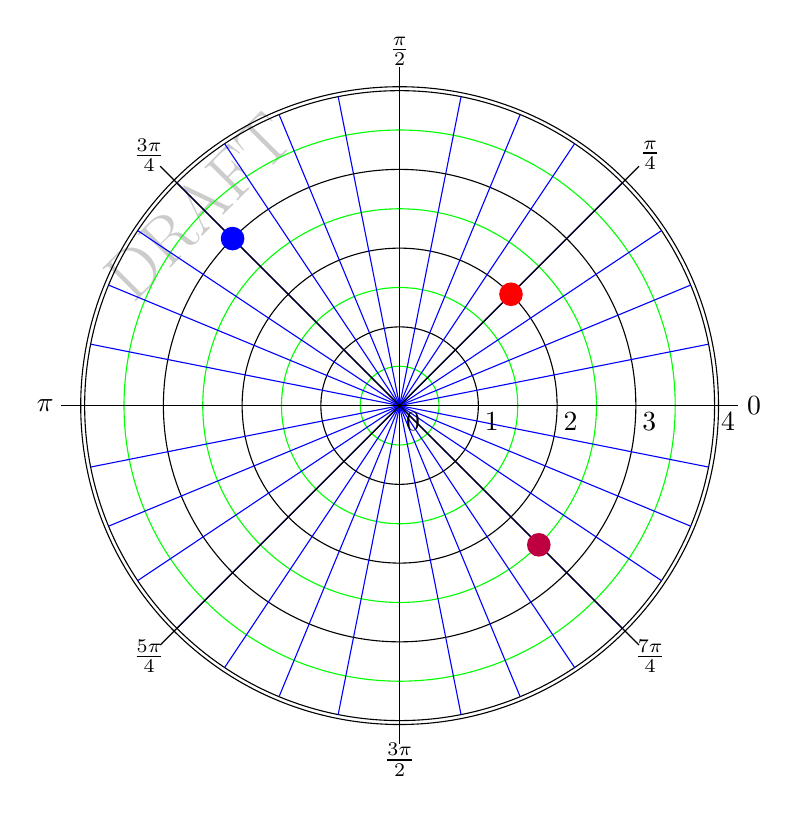
\begin{tikzpicture}[>=latex]
	\foreach \x in {0,...,4,4.05}{\draw (0,0) circle (\x);}
	\foreach \x in {0.5,...,4}{\draw[green] (0,0) circle (\x);}
	\pgfmathparse{360/32}\let\malr=\pgfmathresult
	\foreach \x in {0,\malr,...,360}{\draw[blue,thin](0,0)--(\x:4);}
	\foreach \x in {0,45,...,360}{\draw(0,0)--(\x:4.3);}
	\foreach \x in {0,...,4}{\node at (\x+0.17,-0.2){\x};}
	\foreach \x/\y in {0/0, 45/$\frac{\pi}{4}$, 90/$\frac{\pi}{2}$, 135/$\frac{3\pi}{4}$, 180/$\pi$, 225/$\frac{5\pi}{4}$, 270/$\frac{3\pi}{2}$, 315/$\frac{7\pi}{4}$}
	{\node at (\x:4.5) {\y};}
		\fill[red] (45:2) circle (1.5 mm);
			\fill[blue] (135:3) circle (1.5 mm);
			\fill[purple] (315:2.5) circle (1.5 mm);
\end{tikzpicture} 
\\
$\textcolor{red}{(2,\frac{\pi}{4})}$, $\textcolor{blue}{(3,\frac{3\pi}{4})}$, এবং  $\textcolor{purple}{(2.5,\frac{7\pi}{4})}$ তিনটি বিন্দুকে পোলার গ্রাফ পেপারে প্রদর্শন করা হলো \\
\\ 
\vspace{5cm}
\\
পোলার স্থানাঙ্ক ও কার্তেসীয় স্থানাঙ্কের মধ্যে পার্থক্য\\
\\
কার্তেসীয় স্থানাঙ্ক ব্যবস্থায় যেকোনো একটি বিন্দুকে  কেবলমাত্র একটি নির্দিস্ট ক্রমজোড়ের মাধামে প্রকাশ করা হয় \\
\\
পোলার স্থানাঙ্ক ব্যবস্থায় যেকোনো একটি বিন্দুকে অসংখ্য ক্রমজোড়ের মাধ্যামে প্রকাশ করা সম্ভব\\
\\ 
$(x,y)=\left(\frac{5}{2},\frac{5\sqrt{3}}{2}\right)$ বিন্দুটির পোলার স্থানাঙ্ক নিম্নরূপ\\
\\
$(r,\theta)=\textcolor{green}{(5,\frac{\pi}{3})}=\textcolor{magenta}{(5,-\frac{5\pi}{3})}=\textcolor{purple}{(-5,\frac{4\pi}{3})}=\textcolor{cyan}{(-5,-\frac{2\pi}{3})}$\\
\\ 
কার্তেসীয় গ্রাফ পেপারে পোলার স্থানাঙ্ক \\ 
\\ 
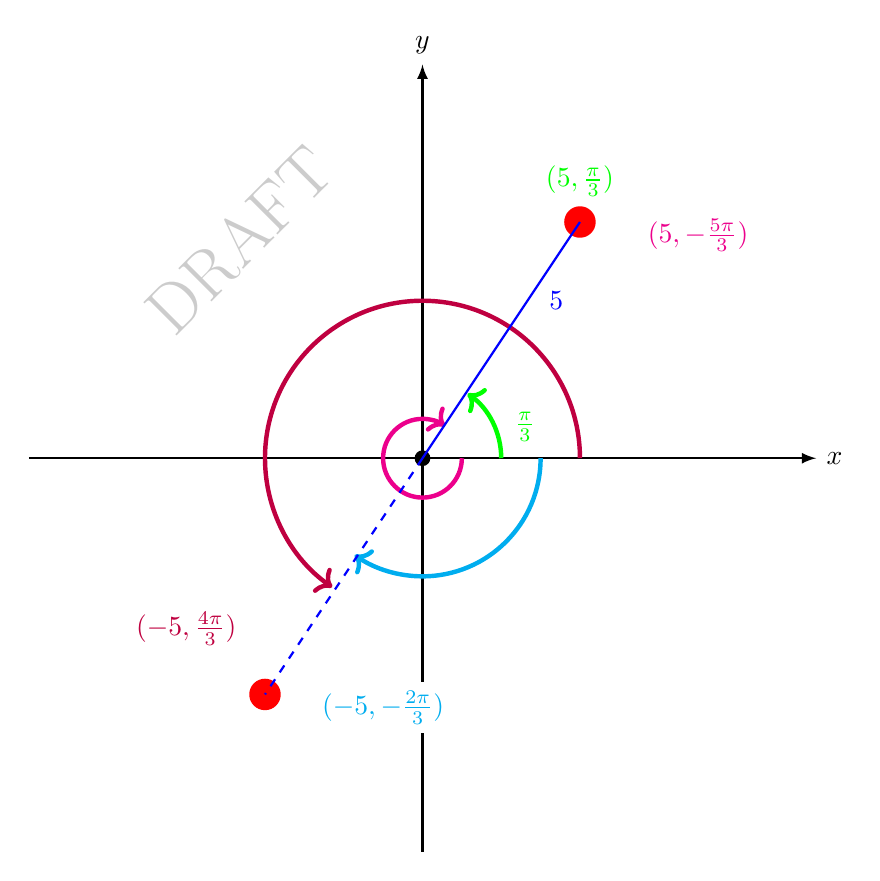
\begin{tikzpicture}[transform shape,scale=1]
	\draw [-latex,thick](-5,0) -- (5,0) node[right] {$x$} coordinate(x axis);
	\draw [-latex,thick](0,-5) -- (0,5) node[above] {$y$} coordinate(y axis);
	\fill[black] (0,0) circle (1 mm);
	\fill[red] (2,3) circle (2 mm);
		\fill[red] (-2,-3) circle (2 mm);
	\node[fill=white,above] at (2,3.2) {$\textcolor{green}{(5,\frac{\pi}{3})}$};
	\node[fill=white,above] at (3.5,2.5) {$\textcolor{magenta}{(5,-\frac{5\pi}{3})}$};
	\node[fill=white,above] at (-3,-2.5) {$\textcolor{purple}{(-5,\frac{4\pi}{3})}$};
	\node[fill=white,above] at (-0.5,-3.5) {$\textcolor{cyan}{(-5,-\frac{2\pi}{3})}$};
	\node at (1.7,2) {$\textcolor{blue}{5}$};
	\node at (1.3,0.4) {$\textcolor{green}{\frac{\pi}{3}}$};	
	\draw[color=green,ultra thick, ->] (1,0) arc (0:55:1cm);
	\draw[color=purple,ultra thick, ->] (2,0) arc (0:235:2cm);
	\draw[color=cyan,ultra thick, ->] (1.5,0) arc (0:-125:1.5cm);
	\draw[color=magenta,ultra thick, ->] (0.5,0) arc (0:-305:0.5cm);
	\draw[thick,blue] (0,0)--(2,3);
	\draw[dashed,thick,blue] (0,0)--(-2,-3);
\end{tikzpicture}
\\
$\textcolor{blue}{x=r\,\,\cos \theta}$,\quad $\textcolor{blue}{y=r\,\,\sin \theta}$ \\
\end{document}